% !TEX root = ../zavrsni_rad.tex

\chapter{Globalno planiranje putanje}
\label{pog:astar}

\section{A* algoritam}

Prije nego NMPC može pratiti putanju, potrebno je tu putanju pronaći. A* algoritam pretražuje diskretiziranu mrežu prostora i pronalazi najkraći slobodan put od starta do cilja.

\subsection{Diskretizacija prostora}

Okolina dimenzija $10 \times 10$ m podijeli se u pravokutnu mrežu s rezolucijom $\delta = 0{,}2$ m po ćeliji, što daje mrežu $51 \times 51 = 2601$ čvorova. Svaka ćelija označena je kao slobodna ili blokirana na osnovu udaljenosti od prepreka:

\begin{equation}
  \text{blokirana}(i,j) = \left\| w_{i,j} - c_k \right\|_2 \leq r_k + r_{rob} + \delta_{inf}
\end{equation}

gdje je $w_{i,j}$ koordinata ćelije u prostoru, $c_k$ centar prepreke, $r_k$ njezin polumjer, $r_{rob} = 0{,}2$ m polumjer robota i $\delta_{inf} = 0{,}2$ m dodatno proširenje prepreke. Ukupno proširenje prepreke iznosi $r_{rob} + \delta_{inf} = 0{,}4$ m --- to znači da se centar robota ne može naći unutar 0,4 m od ruba bilo koje prepreke.

Implementacija u \texttt{src/astar.py}:

\begin{listing}[H]
\begin{minted}{python}
# ukupno proširenje = sigurnosna margina + polumjer robota
inflation = p["astar"]["obstacle_inflation"] + p["robot"]["radius"]  # 0.2 + 0.2 = 0.4 m

for (cx, cy, r) in to_acados_list(obstacles):  # za svaku prepreku (centar + polumjer)
    for i in range(nx):
        for j in range(ny):
            wx, wy = grid_to_world(i, j)        # indeks ćelije → koordinata u prostoru
            # ćelija je blokirana ako joj je centar unutar proširene prepreke
            if (wx - cx)**2 + (wy - cy)**2 <= (r + inflation)**2:
                occupied[i, j] = True
\end{minted}
\caption{Označavanje blokiranih ćelija u \texttt{src/astar.py}}
\end{listing}

\begin{figure}[H]
  \centering
  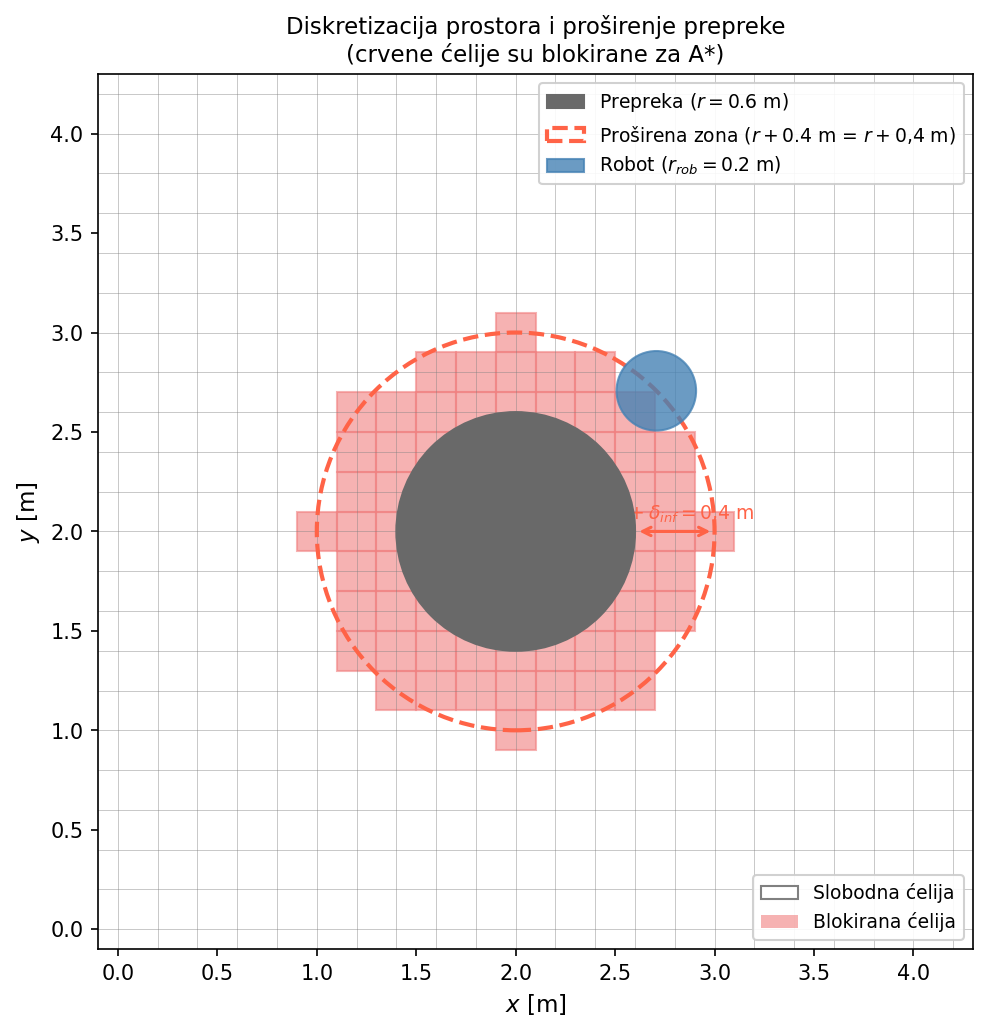
\includegraphics[width=0.75\linewidth]{figures/astar_grid.png}
  \caption{Diskretizacija prostora i proširenje prepreke. Crvene ćelije su blokirane za A* jer im je centar unutar proširene zone (isprekidani krug). Robot (plavi krug) može se kretati samo centrom slobodnih ćelija, što garantira da nikada neće doći u fizički kontakt s preprekom.}
  \label{slk:astar_grid}
\end{figure}

\subsection{Pretraga}

A* koristi prioritetni red i za svaki čvor $n$ prati procjenu ukupnog troška:

\begin{equation}
  f(n) = g(n) + h(n)
\end{equation}

gdje je $g(n)$ stvarni trošak puta od starta do čvora $n$, a $h(n)$ euklidska udaljenost do cilja:

\begin{equation}
  h(n) = \sqrt{(n_x - g_x)^2 + (n_y - g_y)^2}
\end{equation}

Algoritam uvijek proširuje čvor s najmanjim $f(n)$. Euklidska heuristika nikad ne precjenjuje stvarni trošak, što garantira pronalazak optimalnog puta. Susjedi se razmatraju u 8 smjerova --- 4 kardinalna (trošak 1,0) i 4 dijagonalna (trošak $\sqrt{2}$).

Kada A* prođe kroz sve dostupne ćelije i ne pronađe put do cilja, program javlja grešku --- to znači da put ne postoji:

\begin{listing}[H]
\begin{minted}{python}
neighbours = [(-1,0),(1,0),(0,-1),(0,1),       # kardinalni smjerovi
              (-1,-1),(-1,1),(1,-1),(1,1)]       # dijagonalni smjerovi

while open_set:
    _, g, current = heapq.heappop(open_set)     # uzmi čvor s najmanjim f
    if current == goal_g:
        # rekonstruiraj put unatrag
        ...
    for di, dj in neighbours:
        step = np.hypot(di, dj)                 # 1.0 ili sqrt(2)
        new_g = g + step
        if new_g < g_score.get(nb, np.inf):
            f = new_g + heuristic(nb, goal_g)
            heapq.heappush(open_set, (f, new_g, nb))

raise RuntimeError("A*: nema puta od starta do cilja")
\end{minted}
\caption{Jezgra A* pretrage u \texttt{src/astar.py}}
\end{listing}

\begin{figure}[H]
  \centering
  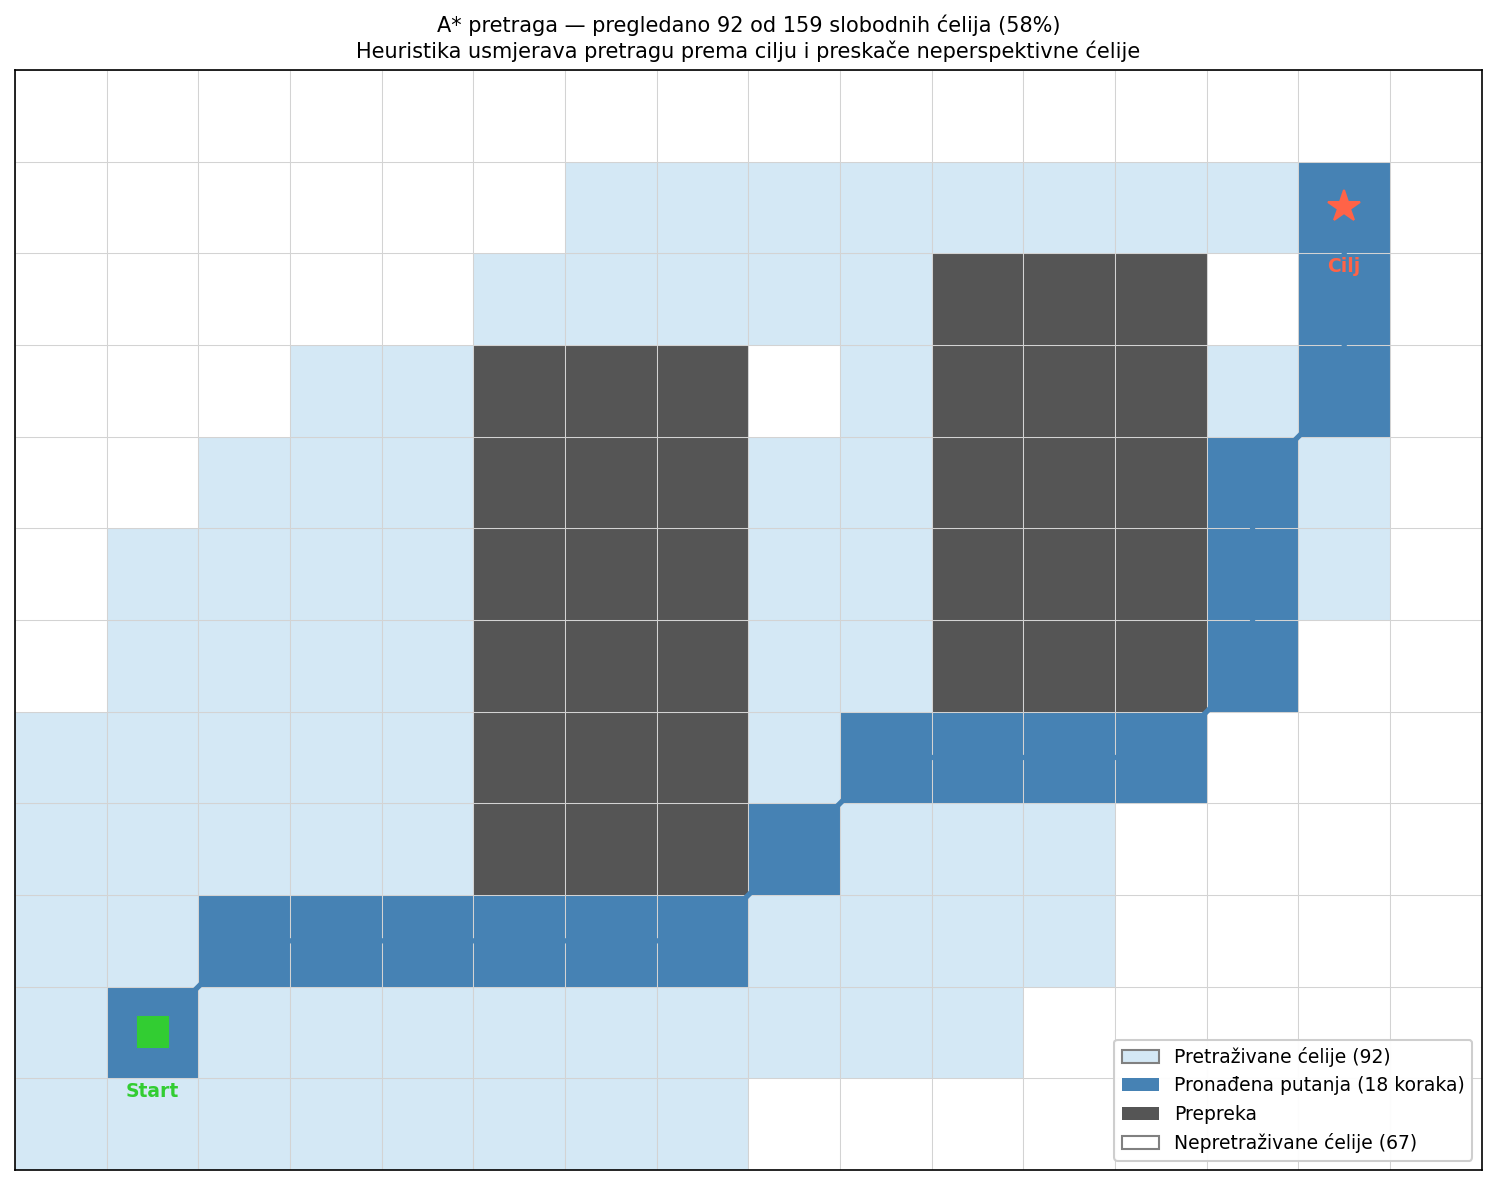
\includegraphics[width=0.90\linewidth]{figures/astar_search.png}
  \caption{Vizualizacija A* pretrage na primjeru mreže s dvije prepreke. Svjetloplavi čvorovi su pretraživani, tamno plavi čvorovi su na pronađenoj putanji, bijeli čvorovi nisu ni razmatrani. Heuristika usmjerava pretragu prema cilju i preskače neperspektivne čvorove.}
  \label{slk:astar_search}
\end{figure}

\subsection{Pravokutne prepreke}

A* radi s kružnim preprekama jer za njih proširenje prepreke ima jasnu geometrijsku interpretaciju. Pravokutne prepreke (korištene u L-hodniku i U-obliku) aproksimiraju se mrežom malih kružnica polumjera 0,2 m, što je razlog opisan u poglavlju~\ref{pog:nmpc} --- acados zahtijeva glatke, derivabilne funkcije za računanje Jacobijana.

\begin{listing}[H]
\begin{minted}{python}
def to_circles(self, r: float = 0.2) -> list[Circle]:
    circles = []
    x = self.x_min + r             # počni od lijevog ruba + polumjer
    while x <= self.x_max:
        y = self.y_min + r         # počni od donjeg ruba + polumjer
        while y <= self.y_max:
            circles.append(Circle(x, y, r))  # dodaj kružnicu u točki (x, y)
            y += r * 1.5           # razmak između kružnica (dovoljno gusto da nema prolaza)
        x += r * 1.5
    return circles
\end{minted}
\caption{Aproksimacija pravokutnika mrežom kružnica u \texttt{src/obstacles.py}}
\end{listing}

\begin{figure}[H]
  \centering
  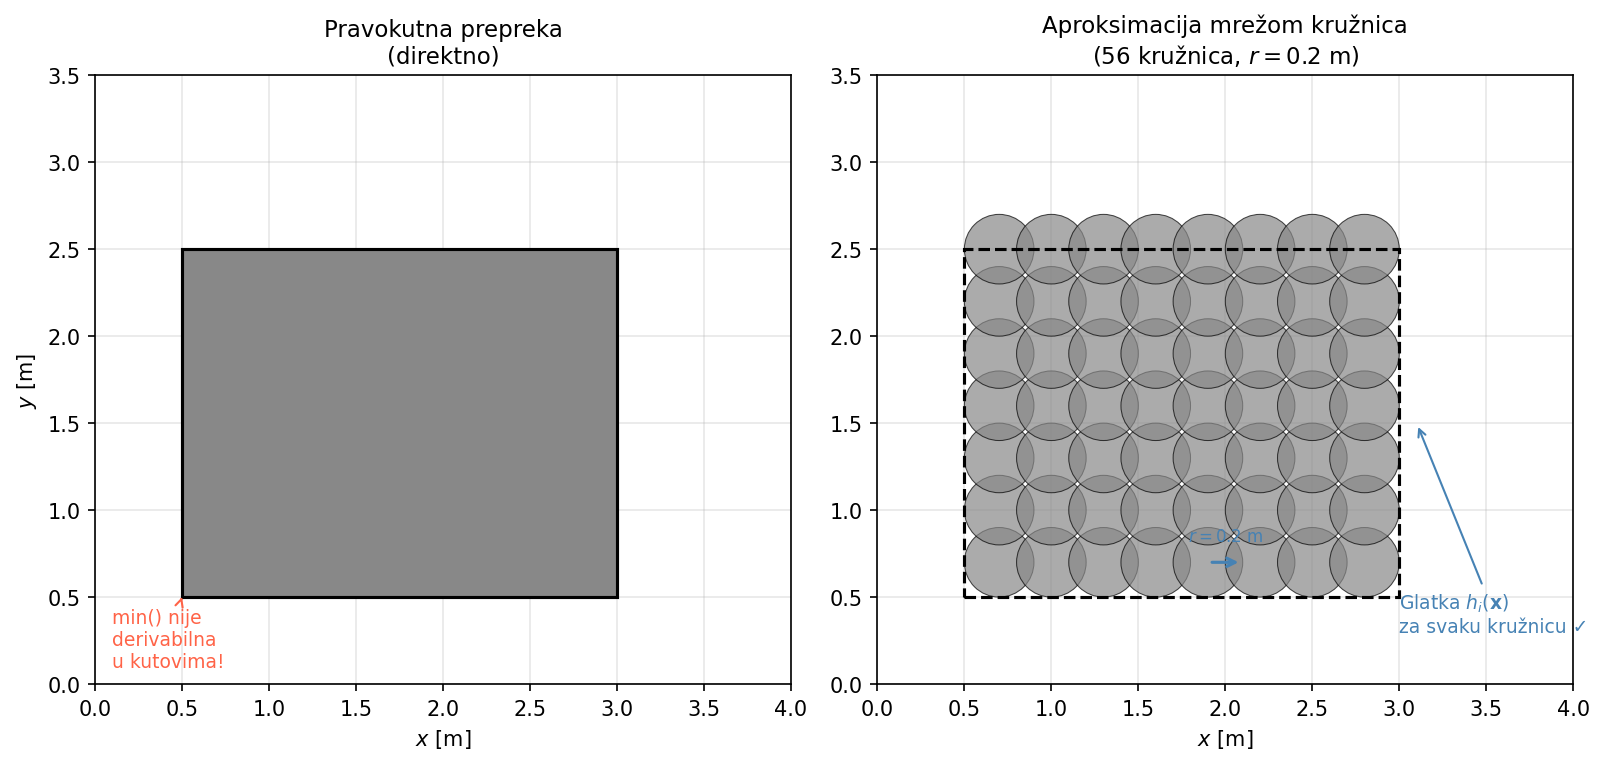
\includegraphics[width=0.95\linewidth]{figures/rect_to_circles.png}
  \caption{Lijevo: pravokutna prepreka direktno --- ograničenje $h(\mathbf{x})$ nije glatko u kutovima pa acados ne može računati Jacobijane. Desno: ista prepreka aproksimirana mrežom kružnica --- svaka kružnica ima glatku $h_i(\mathbf{x})$ pa SQP iteracije rade ispravno.}
  \label{slk:rect_to_circles}
\end{figure}

\section{Izglađivanje putanje}

A* putanja sadrži oštre kutove jer je ograničena rešetkom. Takva putanja nije pogodna kao referenca za NMPC jer zahtijeva nagle promjene smjera. Stoga se izglađuje \textbf{kubičnim B-splineom} koristeći \texttt{scipy.interpolate.splprep}:

\begin{listing}[H]
\begin{minted}{python}
tck, _ = splprep([pts[:, 0], pts[:, 1]], s=0.5, k=3)  # kubični spline, s=0.5
t = np.linspace(0, 1, n_points)                        # 200 jednakomjernih točaka
x_s, y_s = splev(t, tck)
\end{minted}
\caption{Izglađivanje putanje kubičnim splineom u \texttt{src/path\_smoother.py}}
\end{listing}

Parametar izglađivanja $s = 0{,}5$ dopušta B-spline krivulji da ne prolazi točno kroz sve A* točke, nego pronalazi glađu krivu koja eliminira sitne oscilacije rešetke. Rezultat je 200 ravnomjerno raspoređenih točaka duž glatke krivulje.

\begin{figure}[H]
  \centering
  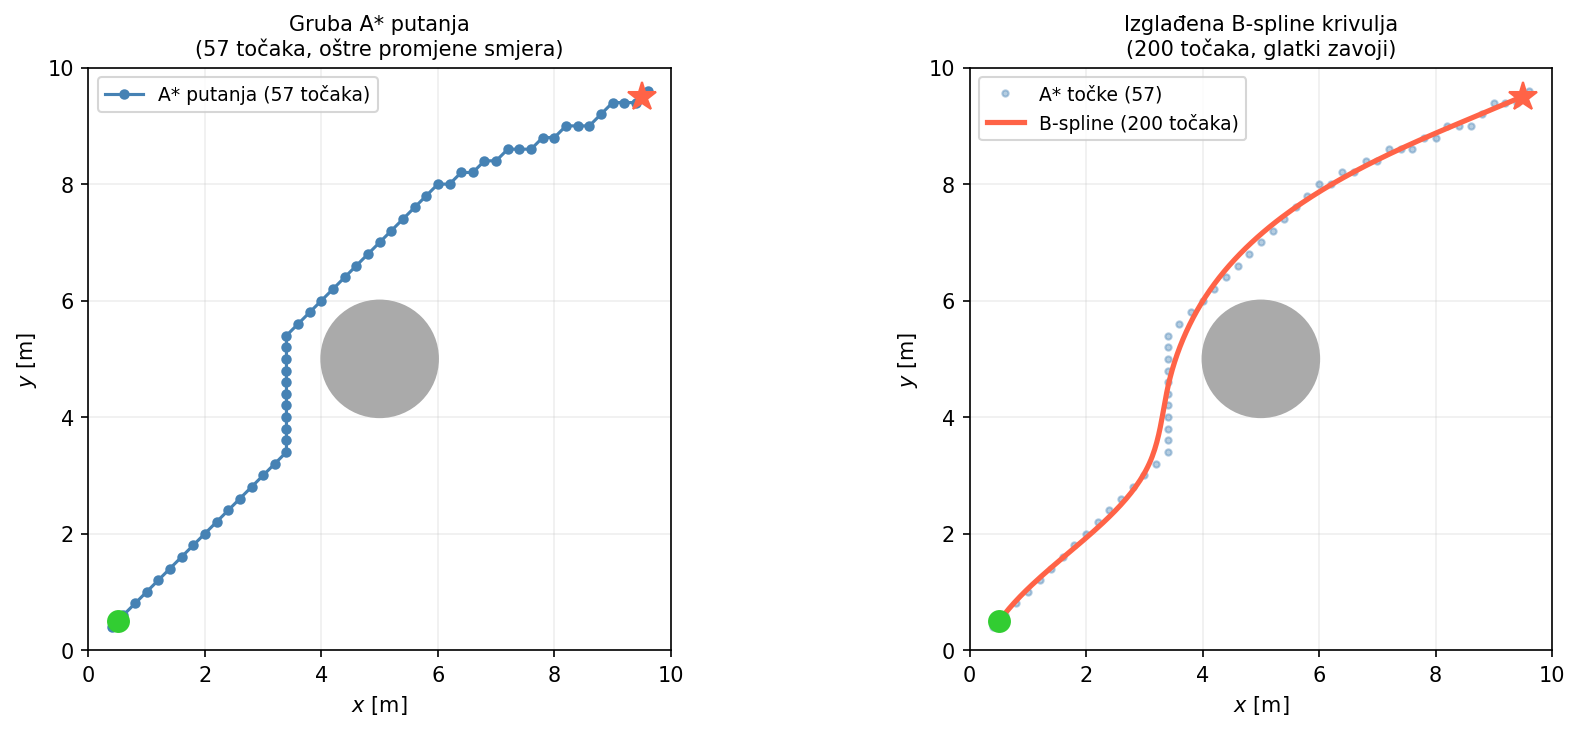
\includegraphics[width=0.95\linewidth]{figures/path_smoothing.png}
  \caption{Lijevo: gruba A* putanja s 57 točaka --- vidljive su oštre promjene smjera karakteristične za rešetku. Desno: ista putanja izglađena B-spline krivuljom s 200 ravnomjerno raspoređenih točaka. Scenarij \texttt{one\_obstacle}, generiran stvarnim kodom iz \texttt{src/astar.py} i \texttt{src/path\_smoother.py}.}
  \label{slk:path_smoothing}
\end{figure}

\section{Profil brzine}

Na ravnim dionicama robot vozi punom brzinom $v_{max} = 1{,}0$ m/s. U zavojima je poželjno usporiti kako bi se smanjila bočna greška praćenja. Referentna brzina računa se iz zakrivljenosti $\kappa$ putanje:

\begin{equation}
  v_{ref}(s) = \frac{v_{max}}{1 + k_{curv} \cdot \kappa(s)}, \qquad k_{curv} = 0{,}5
\end{equation}

gdje se zakrivljenost aproksimira vektorskim produktom uzastopnih segmenata putanje. Profil brzine koristi se isključivo za vizualizaciju referentnog signala u grafovima --- NMPC sam optimizira stvarnu brzinu unutar zadanih ograničenja.

\begin{figure}[H]
  \centering
  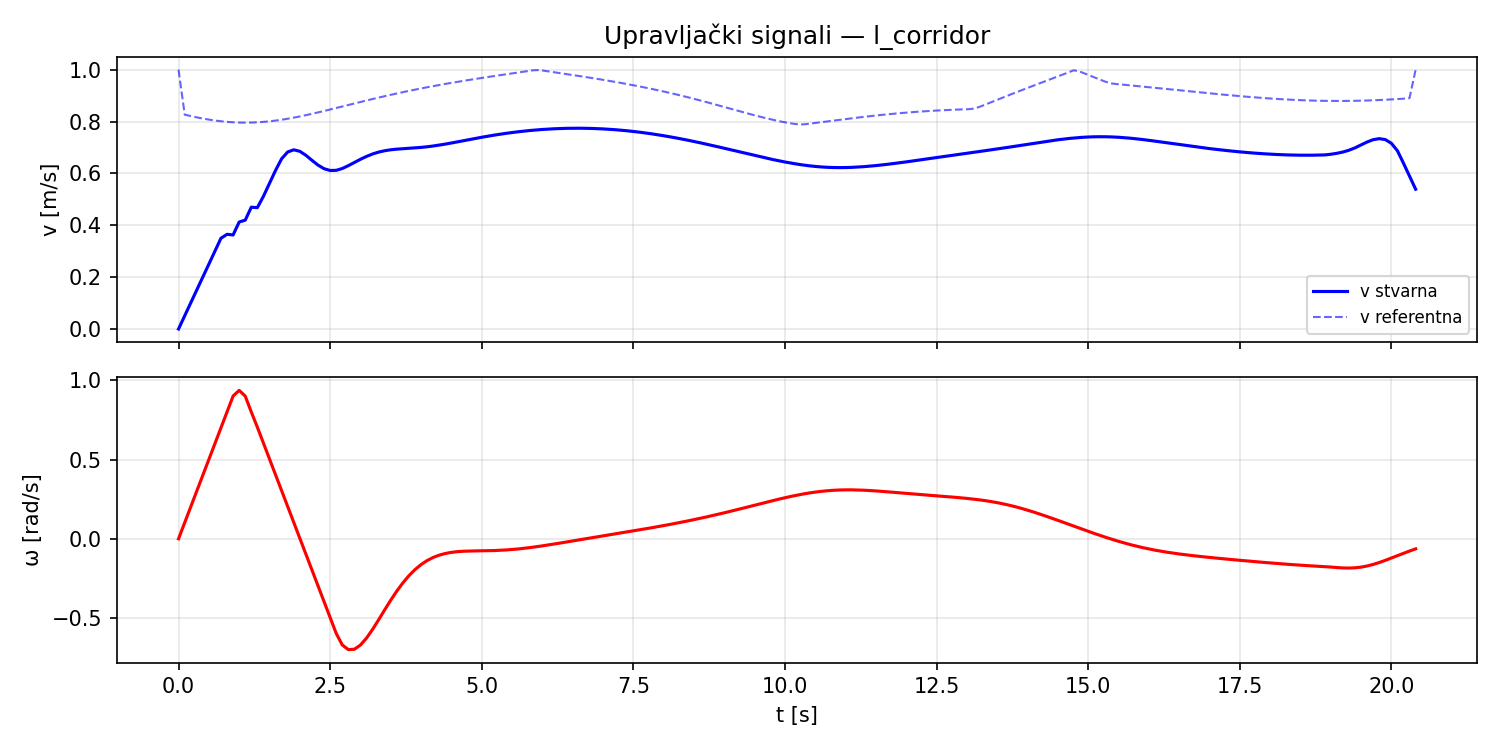
\includegraphics[width=0.90\linewidth]{figures/l_corridor_controls.png}
  \caption{Profil brzine u scenariju L-hodnika. Isprekidana linija prikazuje referentnu brzinu $v_{ref}$ izračunatu prema zakrivljenosti putanje --- vidljivi su padovi na zavojima. Puna linija prikazuje stvarnu brzinu koju NMPC optimizira neovisno o $v_{ref}$.}
  \label{slk:velocity_profile}
\end{figure}
